\documentclass[12pt]{report}
\usepackage[utf8]{inputenc}
\usepackage{fontspec}
\usepackage[a4paper, margin=1in]{geometry}
\usepackage{float}
\usepackage{graphicx}
\usepackage{subfig}

%----------------------------------------------------------
\setromanfont{Times New Roman}

%----------------------------------------------------------


\title{Unveiling the Hardware and Software Implications of Microservices in Cloud and Edge Systems}
\author{Ali Malik}
\date{November 28th, 2022}

\begin{document}

\maketitle

\section*{Background}
As companies make the shift to a more cloud-based architecture, it is important to revisit a very important assumption that has been ubiquitously made...software architecture. One of the most important aspects of these, relatively new, software offerings is their scalability, fault tolerance, concurrency, and availability. All of the previously listed descriptors can be attributed to a very important concept in Computer Science...\textit{distributed systems}. 

What is a distributed system? A distributed system is, like it's name suggests, a system with it's components \textit{distributed} across multiple computers. To help realize a distributed system that is highly available, highly reliable, and highly scalable a very specific software architecture model is used, namely the microservice architecture. Before explaining what the microservice architecture is, it is important to discuss the predecessor, the \textit{monolithic} architecture.

An application which utilizes the monolithic architecture is a very tightly coupled application (shown below), one where components are heavily reliant on one another. That may sound nice, but it actually comes with a slew of problems: complicated feature ingestion, nightmarish upgrades, easily breakable component reliance. To combat this, the microservice architecture was created. Unlike monolithic applications, a microservices oriented application features loosely coupled, sometimes uncoupled, components, that are easy to upgrade. One of the many reasons that microservice architecture is becoming increasing popular is the fact that it promotes a "composable software design", and address the previous problems of updating, deploying, and scaling \cite{article}. 

\begin{figure}[H]
    \centering
    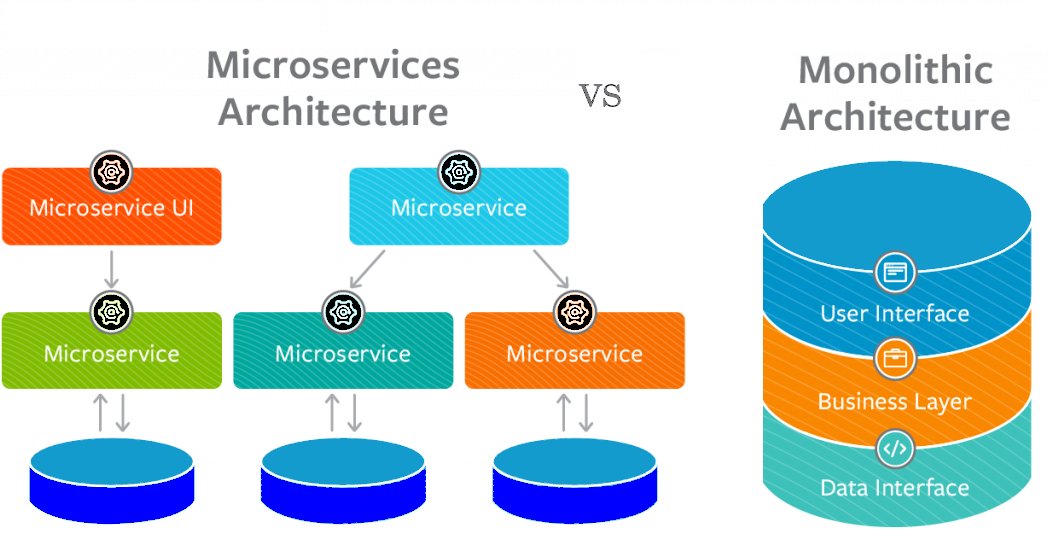
\includegraphics[width=300pt]{images/microVmono.png}
    \caption{Visual depiction of a Monolith vs Microservice Application}
    \label{fig:monoVmicro}
\end{figure}

\section*{Findings}

One of the goals of this study was to take a look at whether microservices are really the way to go. Since microservices are loosely coupled and situated on different machines, high bandwidth and low latency networks become extremely important. Since most distributed systems rely on messaging as the preferred method of communication between components, it makes debugging extremely labor-intensive. Prior to this study, very little was available in terms of cloud systems, so a dependency on open source applications, most of which were monolithic in nature, was created. This study aims at tackling the void that is currently present, "a lack of representative and open-source benchmarks built with microservices..."\cite{article}. 

The result of this study was the creation of the DeathstarBench Suite, which is an "open-sourced set of end-to-end applications built with interactive microservices, representative of popular production online systems."\cite{article}. Each application within this suite adhered to strict design principles such as: representativeness, modularity, extensibility, software heterogeneity, and end-to-end operation. One of the more important aspects is the heterogeneity of code, the reason microservice architecture is so popular is because it allows for a system to have multiple languages across multiple platforms, and capturing that is extremely important if benchmarking microservices is the end goal.

The applications that are included in the DeathstarBench Suite are:
\begin{itemize}
    \item \textit{Social Network}: similar to Facebook
    \item \textit{Media Service}: similar to Netflix
    \item \textit{E-Commerce Store}: similar to Amazon
    \item \textit{Hotel Reservation}
    \item \textit{Banking System}
    \item \textit{IoT Swarm Coordination}
\end{itemize}

Below are the graphical representations of the Social Network and Media Service application, to truly show how interconnected microservice architecture is.

\begin{figure}[H]
    \centering
    \subfloat[\centering label 1]{{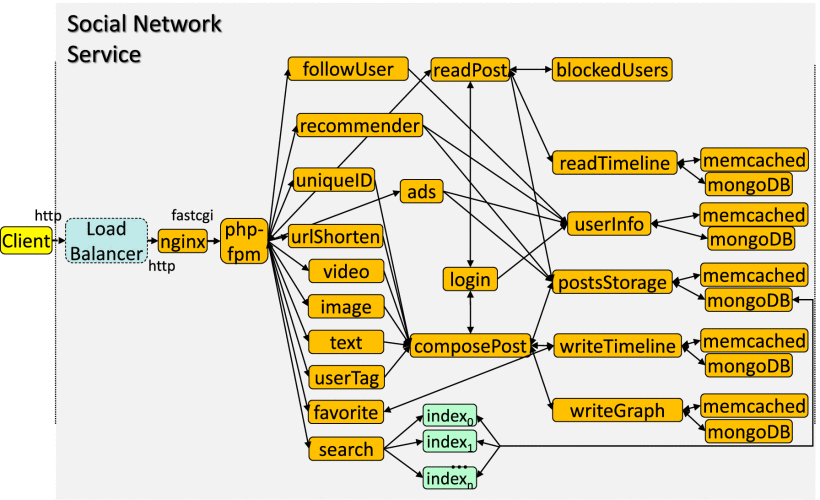
\includegraphics[width=200pt]{images/social_network.png} }}
    \qquad
    \subfloat[\centering label 2]{{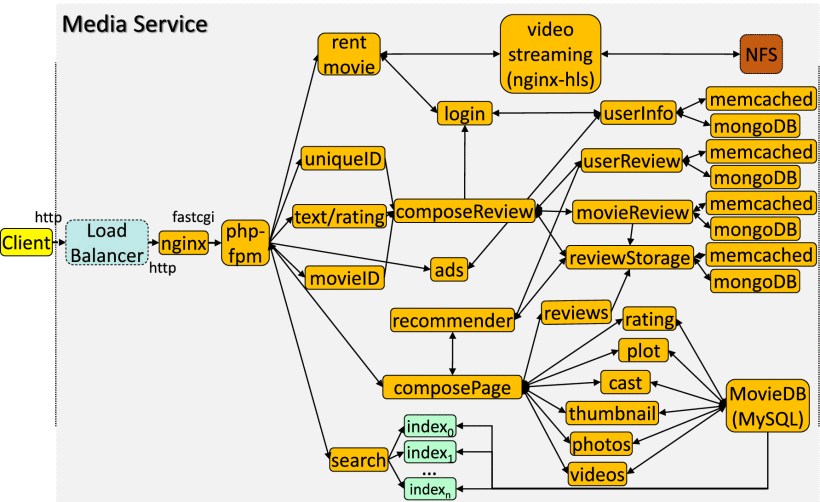
\includegraphics[width=200pt]{images/media_service.png} }}
    \caption{Graph of the microservices for both the Social Networking and Media Service applications}
    \label{fig:graphs}
\end{figure}

These five microservices were evaluated for their implications on cloud hardware based on these five key areas:
\begin{itemize}
    \item Server Design
    \item Networking and OS Overheads
    \item Cluster Management
    \item Serverless Programming Frameworks
\end{itemize}

\subsection*{Server Design}
Firstly, it was quantified how well current datacenters can run microservices and what needs to be changed to meet the strict performance and resource requirements for those very applications. The tail latency (high latencies that infrequent) was measured as load increased for the five microservice applications, as well as, five monolithic applications such as: MongoDB, Xapian, memcached, nginx and Recommender. 

Interestingly enough, as load increases the tail latency for the microservice applications not only increased but also caused quality of service (QoS) violations. While latency did increase for the monolithic applications, those applications didn't encounter nearly as many QoS violations. The heat map below shows the data:

\begin{figure}[H]
    \centering
    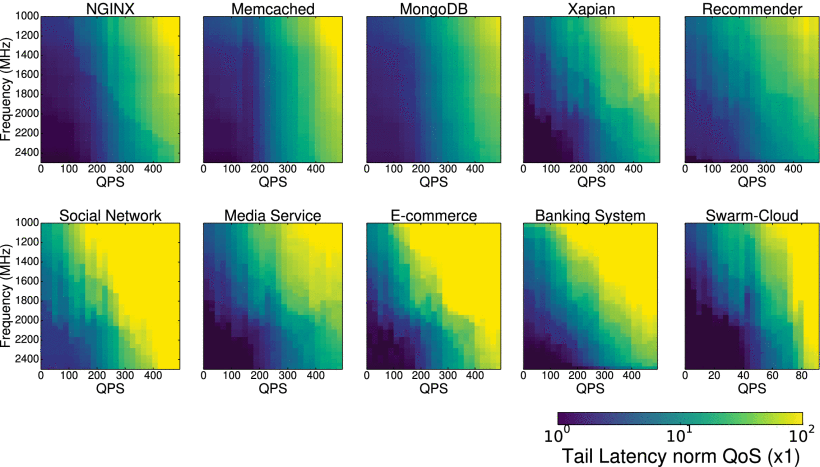
\includegraphics[width=300pt]{images/heat_map_qos.png}
    \caption{Tail Latency with increasing load and decreasing frequency. Traditional monotlithic applications are on top while the microservice architected applications are below.}
    \label{fig:qos_heatmap}
\end{figure}

As observed, the E-Commerce and Social Networking applications are the most sensitive to low frequencies.

\subsection*{Networking and OS Overheads}
As microservices are loosely coupled, communication to/from each service is reliant on some type of messaging queue and RPC or RESTful APIs. Since both the messaging queues and RPC/REST APIs rely on the network, this becomes the bottleneck. For monolithic applications very little time is spent for network processing for the microservices, however, the network processing time accounts for roughly "36.3\% on average, and on occasion over 50\% of the end-to-end latency..."\cite{article}. 

To combat the network bottleneck, a bump-in-the-wire setup is used to achieve hardware acceleration via FPGAs to address the very strict requirements of high throughput and low latency. Using this method, the researchers were able to improve end-to-end tail latency by 43\%.

Below is the topological view of the bump-in-the-wire network, as well as, the effects of hardware acceleration on the end-to-end tail latency.

\begin{figure}[H]
    \centering
    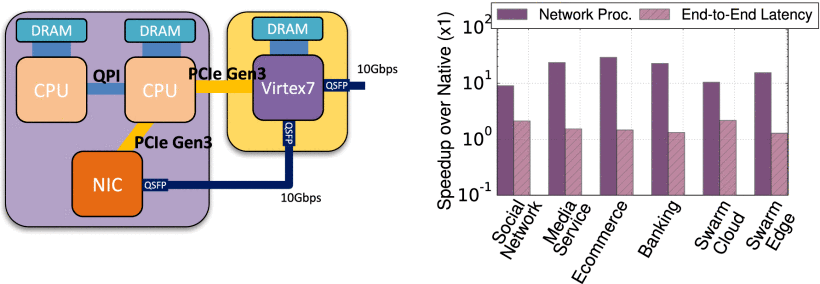
\includegraphics[width=300pt]{images/network.png}
    \caption{On the left is the topological view of the new network. On the right, benefits of the acceleration on end-to-end tail latency.}
    \label{fig:network}
\end{figure}

\subsection*{Cluster Management}
The cluster manager is the entity that is responsible for maintaining the scalability of the application. The issue is that microservices can create a backpressure of QoS violations that cascade their way down causing irregularities in scaling from the cluster manager, resulting in the cluster manager scaling up or scaling down microservices improperly. 

There is a  correlation between a complex dependency graph and the rate at which these issues occur. This naturally leads to microservices suffering a bit when QoS violations cascade down, leading to a longer recovery period simply due to the fact that there are so many components.

Below shows a graph of how monoliths and microservices recover from QoS violations.

\begin{figure}[H]
    \centering
    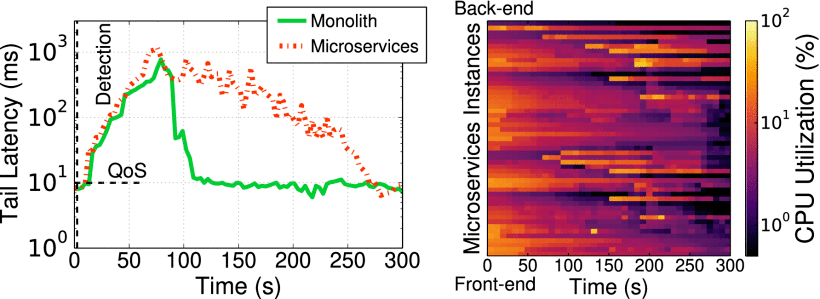
\includegraphics[width=300pt]{images/latency.png}
    \caption{The left shows the time it takes for monoliths and microservices to recover. The right shows the same thing but with auto-scaling measures}
    \label{fig:latency}
\end{figure}

\subsection*{Serverless Programming Frameworks}
The very same applications very testd on AWS' serverless framework...AWS Lambda. Although AWS Lambda is geared towards elastic compute and short bursts of unpredictability of performance remains. In Lambda's case, communication between dependent functions happens via persistent storage, which causes high latency. Another issue is the short lived nature of the VMs running the serverless compute. They're typically designed to run for a couple of minutes and then be terminated. The conclusion being, serverless compute presents different challenges than microservices, but have their specific use cases.

\subsection*{Conclusion}
The DeathstarBench suite calls attention to the widely utilized microservice architecture and also highlights some research areas. In addition, the DeathstarBench suite provides an open-source implementation of various microservice architected applications for academic and professional research.

In the last decade, as cloud computing has gained traction, the research into the foray hasn't evolved accordingly. It is specifically called out in the study, "As cloud software evolves, the direction of such research efforts should also evolve with it." \cite{article}. The study also calls for systems research in this field, while also calling out the importance of hardware-software codesign in cloud applications as they get more complex. 

The biggest takeaway from the study is that current platforms just aren't well suited to the needs of these highly available, reliable, and scalable systems that require extremely low latency and a predictable response. The opportunities and challenges that are presented in this field require a bottom up approach, starting with the servers themselves, optimizing them specifically for microservices. Then moving to networking and addressing the ultra low latency requirements for these systems. 

Finally, to end, as microservices architecture becomes more prevalent and continue to evolve it is increasingly important for the servers, networks, cluster managers, and programming frameworks that they rely on to also evolve hand-in-hand.



\listoffigures
\bibliographystyle{plain}
\bibliography{ref}

\end{document}
